%%%%%%%% ICML 2027 submission (style adapted from ICML 2026 official kit) %%%%%
% Swap icml2027.sty -> official icml2027.sty when the 2027 author kit is released.
\documentclass{article}

\usepackage{microtype}
\usepackage{graphicx}
\usepackage{subcaption}
\usepackage{booktabs}
\usepackage{multirow}
\usepackage{hyperref}
\newcommand{\theHalgorithm}{\arabic{algorithm}}

% Blind review (default). For camera-ready: \usepackage[accepted]{icml2027}
\usepackage{icml2027}

\usepackage{amsmath,amssymb,amsthm}
\usepackage{mathtools}
\usepackage{xcolor}
\usepackage{url}
% algorithm + algorithmic already loaded by icml2027.sty
\usepackage[capitalize,noabbrev]{cleveref}

\newcommand{\pmode}{\pi_{\mathrm{mode}}}
\newcommand{\phat}{\hat{p}}
\newcommand{\rdis}{\rho_{\mathrm{disatt}}}

\theoremstyle{plain}
\newtheorem{proposition}{Proposition}
\theoremstyle{definition}
\newtheorem{definition}{Definition}
\theoremstyle{remark}
\newtheorem{remark}{Remark}

\icmltitlerunning{Pooling Fails; Seed Controls Bound Selector Gains}

\begin{document}

\twocolumn[
\icmltitle{Equal-Budget Prompt Pooling Does Not Beat Self-Consistency---\\
And Seed-Matched Controls Bound Apparent Selector Gains}

\begin{icmlauthorlist}
  \icmlauthor{Anonymous Author}{anon}
\end{icmlauthorlist}
\icmlaffiliation{anon}{Anonymous Institution}
\icmlcorrespondingauthor{Anonymous Author}{anonymous@domain.edu}
\icmlkeywords{reasoning, self-consistency, elicitation, test-time compute, configuration selection}

\vskip 0.3in
]

\printAffiliationsAndNotice{}

\begin{abstract}
Self-consistency (SC) is capped by a modal ceiling $\pmode$. Semantics-preserving
elicitation can change plug-in modes, yet equal-budget configuration-diversified
voting (CDV) need not help. On a crossed sampled-CoT grid (Qwen2.5\,\{1.5B,3B,7B\},
Llama-3.2-3B; MATH-500, GSM8K, GSM-Symbolic; $\{c_0,c_1,c_2\}$) we find:
\textbf{(C1)} plug-in $\pmode$ spreads ${>}3$\,pp on several cells (largest on
GSM-Symbolic); \textbf{(C2)} token-matched equal-budget CDV shows no positive
lift vs.\ SC (mean $\Delta{\approx}{-}0.7$\,pp; pooled CI crosses zero);
\textbf{(C3)} a pre-specified conditional-diversify rule gains
${\approx}{+}2.3$\,pp vs.\ SC@$N$ over $14$ cells
(CI~$[{+}1.1,{+}3.7]$), but on the $6$ multi-seed cells seed-substitution
recovers ${\approx}{+}2.0$\,pp and config$-$seed is ${\approx}{-}0.4$\,pp
(CI~$[{-}1.2,{+}0.3]$), so we \emph{cannot distinguish} configs from seeds.
An independent margin-split still beats SC; probe-then-commit costs
${\approx}1.6\times$ SC@$N$ tokens (${\approx}0.53\times$ always-3).
Seed-null oracles (${\approx}4.5$\,pp) match cross-config plug-in oracles.
We do \emph{not} claim elicitation recovery; the contribution is a careful CDV
negative plus a protocol warning against confounding selectors with denoising.
\end{abstract}

% ============================================================================
\section{Introduction}
\label{sec:intro}
% ============================================================================

Progress in language-model reasoning is increasingly mediated by how a model
\emph{selects} an answer under sampling. Compute-optimal test-time scaling bins
items by estimated difficulty~\citep{snell2024scaling}; adaptive
self-consistency stops when a vote looks decided~\citep{aggarwal2023adaptive,li2024esc};
and analyses that explain why extra samples stop helping bound selection by the
\emph{modal-hit rate} $\pmode$---the fraction of items whose plurality answer is
correct~\citep{brown2024monkeys,blendasc2025,certifiedsc2025,bay2026modal}.
More i.i.d.\ samples estimate the mode of a \emph{fixed} answer distribution more
precisely; they cannot change which class is modal
(\cref{prop:iid-frozen}). That fact invites three linked questions the
modal-ceiling literature leaves open for sampled chain-of-thought:

\begin{enumerate}\itemsep1pt
  \item[\textbf{C1.}] Does semantics-preserving elicitation change the mode, so
    $\pmode$ is a model--prompt property rather than a model constant?
  \item[\textbf{C2.}] Does spreading a fixed completion-token budget across
    configurations (equal-budget CDV) raise $\pmode$ above single-configuration
    SC?
  \item[\textbf{C3.}] Over a multi-config pool, does a \emph{pre-specified}
    held-out rule beat SC@$N$---and does that lift survive seed-substitution
    and SC@$3N$ controls that match sample count?
\end{enumerate}

Prompt sensitivity of \emph{item difficulty} is already established on
log-prob-scored suites~\citep{brittlebench2026,tee2026} and for unstable hardness
labels~\citep{hardunreached2026}. Those works do not measure whether sensitivity
reaches the \textbf{mode} under \textbf{sampled} CoT, nor do they require
seed-matched controls before attributing multi-prompt gains to elicitation.

\paragraph{What we find.}
\textbf{C1:} plug-in spreads can exceed a $c_0$ seed-null; only $2/6$
multi-seed cells clear both ${>}3$\,pp and a seed-permutation test at
$\alpha{=}0.05$ (largest Symbolic cells still await seeds).
\textbf{C2:} equal-budget CDV shows no positive lift
($\Delta{\approx}{-}0.7$\,pp; CI crosses zero).
\textbf{C3:} conditional diversify gains ${\approx}{+}2.3$\,pp vs.\ SC@$N$,
but config$-$seed and config$-$SC@$3N$ CIs both cross zero on controlled
cells; margin-split and drop-$c_2$ ablations refine rather than reverse this.
Seed-null oracles (${\approx}4.5$\,pp) match cross-config plug-in oracles.

\paragraph{Contributions.}
\begin{enumerate}\itemsep1pt
  \item \textbf{Measurement protocol.} Seed-null, seed-substitution, SC@$kN$,
    margin-split, probe-then-commit tokens, and seed-calibrated P4.
  \item \textbf{C2.} Equal-budget CDV: no positive lift; drop-$c_2$ /
    quality-weighted ablations show $c_2$ is a quality confound.
  \item \textbf{C1.} Selective plug-in $\pmode$ spreads vs.\ a seed-permutation
    null where seeds exist.
  \item \textbf{C3.} Selector gains vs.\ SC@$N$ do not survive seed-matched
    controls on controlled cells; compute cost is ${\approx}1.6\times$ SC@$N$.
\end{enumerate}

\paragraph{Positioning.}
We do not claim first discovery of prompt
sensitivity~\citep{brittlebench2026,tee2026,prompteval2024,sclar2024formatspread}.
The delta is modal CoT measurement, a budget-matched pooling test with honest
uncertainty, and seed-matched controls that show multi-prompt ``selection''
gains are easily confounded with denoising. Extended related work:
\cref{app:related}.

\section{Method}
\label{sec:method}
% ============================================================================

A single sampling corpus supports every quantity offline: no training and no
extra generation for CDV.

\paragraph{Notation.}
For each cell $(i,m,c,s)$ we draw $N$ chains, extract and canonicalise answers,
and record $k_{imcs}$ correct. Write $\phat_{imcs}=k/N$ and the Haldane logit
$z=\log\frac{k+1/2}{N-k+1/2}$. An \emph{elicitation configuration} perturbs
everything except mathematical content. Core set $\{c_0,c_1,c_2\}$:
\begin{itemize}\itemsep1pt
  \item $c_0$: neutral system (``helpful assistant''), zero-shot CoT, $T{=}0.8$;
  \item $c_1$: expert-mathematician system prompt; else as $c_0$;
  \item $c_2$: family-minimal / default-system rendering (audited per family).
\end{itemize}
Parse ($c_3$), few-shot, and temperature axes are separate; $c_5$ appears only in
temperature-diversified SC (B4).

\paragraph{Modal ceiling.}
Plurality class $a^\star$ over $N$ samples; $\pmode(m,c)$ is the fraction of
items with $a^\star$ correct. Gap: $\mathrm{pass@}N-\pmode$. We measure
$\pmode$ ourselves~\citep{brown2024monkeys,bay2026modal}.

\paragraph{Supporting GLMM / moments.}
Crossed binomial GLMM following~\citet{tee2026,prompteval2024}; primary variance
tables report both method-of-moments shares on Haldane logits and VB-GLMM shares
with bootstrap CIs. Seed replicates at $c_0$ supply the noise floor and $r_{mm}$
for disattenuation $\rdis=\rho_{\mathrm{raw}}/r_{mm}$. Hard-subset Jaccard across
configs vs.\ seeds measures excess instability.

\paragraph{CDV (tested policy).}
Split completion-token budget $B$ evenly across
$\mathcal{C}_{\mathrm{use}}=\{c_0,c_1,c_2\}$, pool answer classes, return plurality
(\cref{alg:cdv}). Budgets are matched on \emph{actual} completion tokens
(early stop / length accounted for in the offline allocator). Compare to SC and
temperature-diversified SC. Primary test P5/F3: plug-in $\pmode(\mathrm{CDV})$
vs.\ $\pmode(c_0)$, with item-clustered bootstrap CIs and a pre-specified
equivalence margin $\delta{=}1$\,pp (CI-based TOST; reported even when
inconclusive).

\begin{algorithm}[t]
\caption{Configuration-Diversified Voting (CDV)}
\label{alg:cdv}
\begin{algorithmic}[1]
\REQUIRE item $i$, model $m$, token budget $B$, set $\mathcal{C}_{\mathrm{use}}$
\STATE $b \gets B / |\mathcal{C}_{\mathrm{use}}|$
\STATE $P \gets \emptyset$
\FOR{$c \in \mathcal{C}_{\mathrm{use}}$}
  \STATE draw chains from $(i,m,c)$ until cumulative output tokens reach $b$; add classes to $P$
\ENDFOR
\STATE \textbf{return} $\arg\max_{a}\#\{a\in P\}$
\end{algorithmic}
\end{algorithm}

% ============================================================================

% ============================================================================
\section{Elementary Observations}
\label{sec:formal}
% ============================================================================

We record only elementary facts needed to interpret C1/C2---not a standalone
theory contribution. Proofs are immediate; the empirics test the premises.

\begin{definition}[Modal hit and ceiling]
Fix model $m$, configuration $c$, and item $i$. Let $P_{i,m,c}$ be the
distribution over canonical answer classes induced by sampling chains under
$(m,c)$. Write $\mathrm{mode}(P)$ for a plurality class (ties broken by a fixed
rule). The item is a \emph{modal hit} if $\mathrm{mode}(P_{i,m,c})$ is correct.
Then $\pmode(m,c)$ is the fraction of items that are modal hits.
\end{definition}

\begin{proposition}[i.i.d.\ resampling cannot move a fixed mode]
\label{prop:iid-frozen}
If chains are drawn i.i.d.\ from a fixed $P_{i,m,c}$, then as $N\to\infty$ the
empirical plurality converges to $\mathrm{mode}(P_{i,m,c})$. Increasing $N$
cannot change the population mode; it only reduces estimation error of that mode.
\end{proposition}

\begin{proposition}[Mixture modes need not raise modal correctness]
\label{prop:mixture-not-monotone}
Let $\{P_c\}_{c\in\mathcal{C}}$ be configuration-conditional answer
distributions and let $Q=\sum_{c} w_c P_c$ be any mixture with $w_c\ge 0$,
$\sum_c w_c=1$ (equal-budget CDV is the finite-sample analogue).
Nothing forces $\mathbf{1}[\mathrm{mode}(Q)\ \mathrm{correct}] \ge
\mathbf{1}[\mathrm{mode}(P_{c_0})\ \mathrm{correct}]$ itemwise. In particular,
if moving from $c_0$ to $c$ promotes an incorrect class into the plurality more
often than it demotes one (net-destructive reordering), the mixture can
\emph{lower} modal correctness relative to $c_0$.
\end{proposition}

\begin{proposition}[Margin gate for a beneficial config change]
\label{prop:margin-gate}
Fix item $i$ and write $p_c(a)$ for the mass of canonical class $a$ under
configuration $c$. Let $a^\star$ be correct and $b$ any incorrect competitor.
A change $c_0\to c$ can be corrective only if $p_{c_0}(a^\star)\le p_{c_0}(b)$
and $p_c(a^\star)>p_c(b)$ (up to ties). Equivalently, a flip requires the
$\ell_\infty$ change in class masses to exceed half the source top-two margin
$m_{c_0}=(p_{c_0}(a_{(1)})-p_{c_0}(a_{(2)}))$. Corrective mass is therefore
concentrated on small-margin items---the regularity we measure
descriptively---while destructive flips remain free whenever the correct class
is only narrowly modal under $c_0$. The proposition is symmetric in direction
and does not by itself explain CDV's sign.
\end{proposition}

\begin{remark}
C1 asks whether $P_{i,m,c}$ itself changes with $c$ enough that $\pmode(m,c)$
moves. C2 asks whether a particular mixture policy improves $\pmode$.
\cref{prop:iid-frozen} explains why C2 is interesting;
\cref{prop:mixture-not-monotone,prop:margin-gate} explain why C2 can fail even
when C1 holds, and where reordering should concentrate. Our experiments
instantiate both. These are interpretive elementary facts, not a standalone
theory contribution.
\end{remark}


\section{Experimental Setup}
\label{sec:setup}
% ============================================================================

\paragraph{Models.}
\texttt{Qwen/Qwen2.5-\{1.5B,3B,7B\}-Instruct}~\citep{qwen25,qwen2} and
\texttt{meta-llama/Llama-3.2-3B-Instruct}. Inference with Hugging Face
\texttt{float16}, \texttt{device\_map=auto}, on $1$--$2\times$ NVIDIA T4 (16\,GB).
Precision control: NF4 4-bit on 1.5B/3B MATH-500 only.

\paragraph{Benchmarks.}
MATH-500~\citep{math500} (headline; 200-item subsample), GSM8K~\citep{cobbe2021gsm8k}
(secondary; contamination risk~\citep{zhang2024gsm1k}), and GSM-Symbolic
main/p2~\citep{mirzadeh2025gsmsymbolic} (150 items; stress test). Fixed item-index
files are shipped with the harness.

\paragraph{Sampling.}
Strategy \texttt{configured\_sampling}, $N{=}24$ chains/item (O2: $N{=}64$ on
Qwen2.5-3B$\times$MATH-500$\times\{c_0..c_3\}$), $T{=}0.8$, $\mathrm{top\_p}{=}0.95$,
\texttt{max\_new\_tokens}${=}1024$. Seeds $\{0,1,2\}$ at $c_0$ for Qwen ladder
noise floors; headline table uses seed~$0$. Answers: extract then symbolic
canonicalisation; extraction-failure rates logged in T1/T2.

\paragraph{Corpus.}
$67$ run directories ($61$ fp16 + $6$ 4-bit); \texttt{tab1\_setup.csv} lists
$66$ fp16 graded rows used in the primary tables. Analysis:
\texttt{python -m src.analysis.paper} with VB-GLMM and item-clustered bootstrap
($B{=}1000$). Numbered figures/tables plus depth-stability,
transition-persistence, selection, and C3-control CSVs ship in
\texttt{paper\_artefacts/} and \texttt{paper/tables/}.

\paragraph{Estimand vs.\ plug-in.}
The population target is $\pmode(m,c)$ under $P_{i,m,c}$. Reported tables are
maj@$N$ plug-ins. Depth-stability curves (prefix-$N$ agreement with full-$N$
modes on O2 cells) quantify how often the estimated mode flips as $N$ grows.

\paragraph{Predictions (protocol in code supplement).}
\textbf{Confirmatory:} P4 (plug-in $\pmode$ range ${>}3$\,pp); P5 (token-matched
CDV does not beat SC). \textbf{Exploratory:} whether conditional diversify beats
SC@$N$; whether that lift survives seed-substitution / SC@$3N$; P1, P7,
oracle-recovery \%, transfer panels. We do not claim a public registry timestamp.

% ============================================================================
\section{Results}
\label{sec:results}
% ============================================================================

Unless noted, numbers are maj@$N$ plug-ins for $\pmode$ at seed~$0$ from
\texttt{tab2\_main\_accuracy.csv}, with item-clustered bootstrap CIs
($B{=}1000$) on primary CDV and selection contrasts. For
Qwen2.5-3B$\times$MATH-500 the loader keeps the deeper O2 cells ($N{=}64$) over
$N{=}24$ duplicates.

\paragraph{Reading order.} We report C1 (where ceilings move), C2 (equal-budget
CDV negative), C3 (selection with seed-substitution / SC@$3N$ controls), then
the descriptive reordering panel. Supporting variance/transfer panels are in
\cref{app:extra-figs}. Scope is the models, prompts, and benchmarks below---not
a universal claim about all configuration diversity.

\begin{table}[t]
\centering
\caption{Result card (plug-in maj@$N$ unless noted).}
\label{tab:result-card}
\small
\setlength{\tabcolsep}{3pt}
\resizebox{\linewidth}{!}{%
\begin{tabular}{@{}lll@{}}
\toprule
ID & Comparison & Finding \\
\midrule
C1 & Config $\pmode$ & $2/6$ cells survive seed-permutation P4 \\
C2 & CDV vs.\ SC & $\Delta{\approx}{-}0.7$\,pp; CI crosses 0 \\
C3 & Cond.\ div.\ vs.\ SC@$N$ & $+2.3$\,pp (14 cells) \\
C3ctl & Seed-sub / SC@$3N$ & Indistinguishable on 6 cells \\
Null & Seed oracle & ${\approx}4.5$\,pp $\approx$ config oracle \\
\bottomrule
\end{tabular}}
\end{table}

\subsection{Modal ceilings across configurations (Q1)}
\label{sec:results-ceiling}

\begin{table}[t]
\centering
\caption{Plug-in $\pmode$ (\%; maj@$N$) by configuration, seed~$0$, fp16.
$N{=}24$ except Qwen2.5-3B$\times$MATH-500 ($N{=}64$, O2). Range $=\max-\min$
over $c_0$--$c_2$ in percentage points. Bold: P4 supported ($>3$\,pp).}
\label{tab:main-acc}
\small
\setlength{\tabcolsep}{3.5pt}
\begin{tabular}{llrrrr}
\toprule
Model & Dataset & $c_0$ & $c_1$ & $c_2$ & Range \\
\midrule
Qwen2.5-1.5B & GSM8K & 74.5 & 73.5 & 68.0 & \textbf{6.5} \\
Qwen2.5-1.5B & MATH-500 & 56.0 & 54.0 & 57.0 & 3.0 \\
Qwen2.5-3B & GSM8K & 91.0 & 90.5 & 91.0 & 0.5 \\
Qwen2.5-3B & MATH-500$^{\dagger}$ & 76.0 & 76.5 & 75.5 & 1.0 \\
Qwen2.5-7B & GSM8K & 94.5 & 93.5 & 88.0 & \textbf{6.5} \\
Qwen2.5-7B & MATH-500 & 82.0 & 80.0 & 81.5 & 2.0 \\
Llama-3.2-3B & GSM8K & 89.9 & 88.5 & 87.0 & 2.9 \\
Llama-3.2-3B & MATH-500 & 59.0 & 59.5 & 58.5 & 1.0 \\
\midrule
Qwen2.5-1.5B & Sym.\ main & 60.7 & 57.3 & 59.3 & \textbf{3.3} \\
Qwen2.5-1.5B & Sym.\ p2 & 29.3 & 27.3 & 27.3 & 2.0 \\
Qwen2.5-3B & Sym.\ main & 90.0 & 82.7 & 79.3 & \textbf{10.7} \\
Qwen2.5-3B & Sym.\ p2 & 66.0 & 65.3 & 64.0 & 2.0 \\
Qwen2.5-7B & Sym.\ main & 87.3 & 81.3 & 74.0 & \textbf{13.3} \\
Qwen2.5-7B & Sym.\ p2 & 81.3 & 80.7 & 75.3 & \textbf{6.0} \\
\bottomrule
\end{tabular}\\[2pt]
{\footnotesize $^{\dagger}$O2 deep-$N$ cells retained over $N{=}24$ duplicates.}
\end{table}

\textbf{P4 is supported on several cells, not universally.}
Spreads exceed 3\,pp on 1.5B/7B GSM8K (both 6.5\,pp) and on GSM-Symbolic main for
all three Qwen sizes (3.3 / 10.7 / 13.3\,pp), plus 7B Symbolic p2 (6.0\,pp).
3B GSM8K (0.5\,pp) and Llama GSM8K (2.9\,pp) miss the gate; MATH-500 aggregate
ranges stay $\le 3$\,pp. \paragraph{Seed-calibrated P4.}
On the six multi-seed cells, mean $c_0$ seed-to-seed $\pmode$ range is
${\approx}1.5$\,pp vs.\ mean config range ${\approx}3.3$\,pp. A seed-null
permutation (resample three $c_0$ seed plug-ins; one-sided
$p{=}\Pr[\mathrm{seed\text{-}range}\ge\mathrm{config\text{-}range}]$) leaves
only \textbf{2/6} cells that both exceed $3$\,pp and reject the seed null at
$\alpha{=}0.05$ (1.5B and 7B GSM8K). 3B MATH-500 has seed range $>$ config
range. Table~\ref{tab:main-acc} is therefore a \emph{plug-in} comparison;
Symbolic's large spreads still lack seeds. Large spreads are often
$c_0{>}c_1,c_2$ quality gaps (\cref{fig:ceiling}).

\begin{figure}[t]
\centering
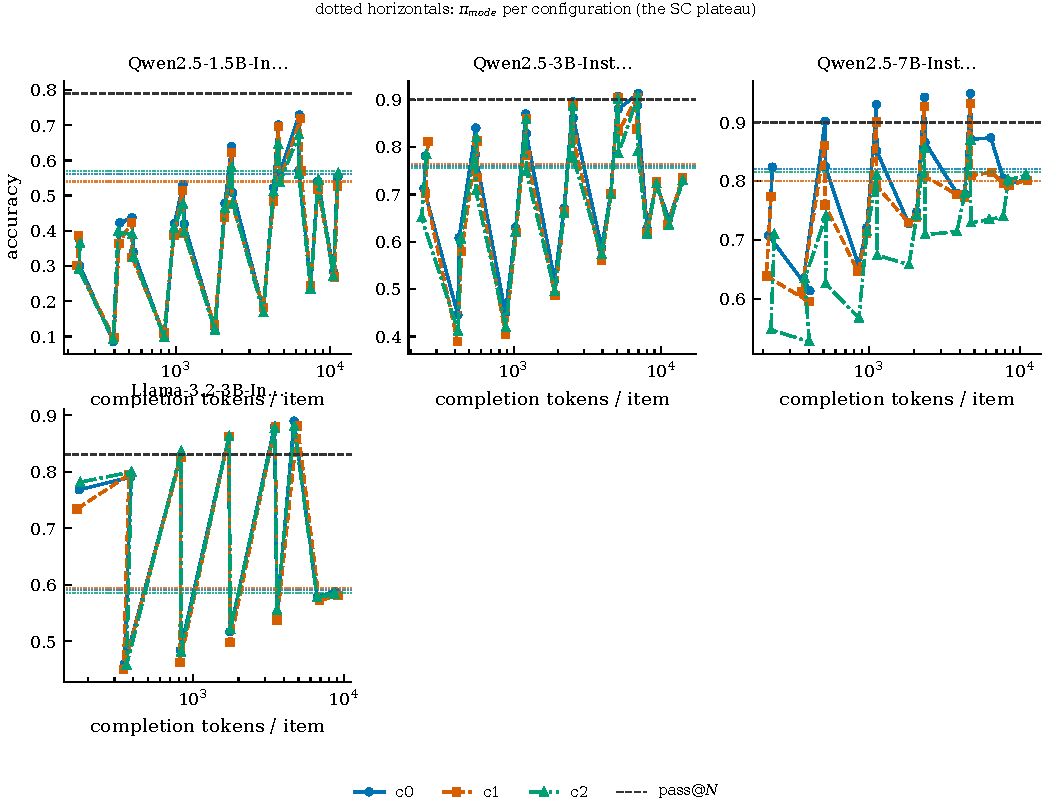
\includegraphics[width=\linewidth]{figures/fig4_ceiling_vs_coverage.pdf}
\caption{Modal ceiling vs.\ coverage (artefact F4).}
\label{fig:ceiling}
\end{figure}

\subsection{Equal-budget CDV does not raise the plateau (C2)}
\label{sec:results-cdv}

O2 on Qwen2.5-3B$\times$MATH-500 at $N{=}64$ gives maj@$64$ of
76.0 / 76.5 / 75.5 / 76.4\% under $c_0$--$c_3$. Equal-budget token-matched CDV
over $\{c_0,c_1,c_2\}$ (\cref{fig:cdv}; Table~T5) shows \textbf{no positive
lift}: mean $\Delta{\approx}{-}0.7$\,pp across $14$ cells at the largest matched
budget; a pooled normal approximation gives CI ${\approx}[{-}1.7,{+}0.3]$\,pp.
Per-cell TOST at $\delta{=}1$\,pp is inconclusive everywhere. CDV stays near SC
and below oracle best-single / coverage bounds. Some configs (notably $c_2$)
are weaker than $c_0$ on high-spread cells, so pooling mixes unequal qualities;
we do not claim all diversity schemes fail---only that this equal-budget allocator
does not demonstrate a lift. Title/conclusion language matches this weaker claim.

\begin{figure}[t]
\centering
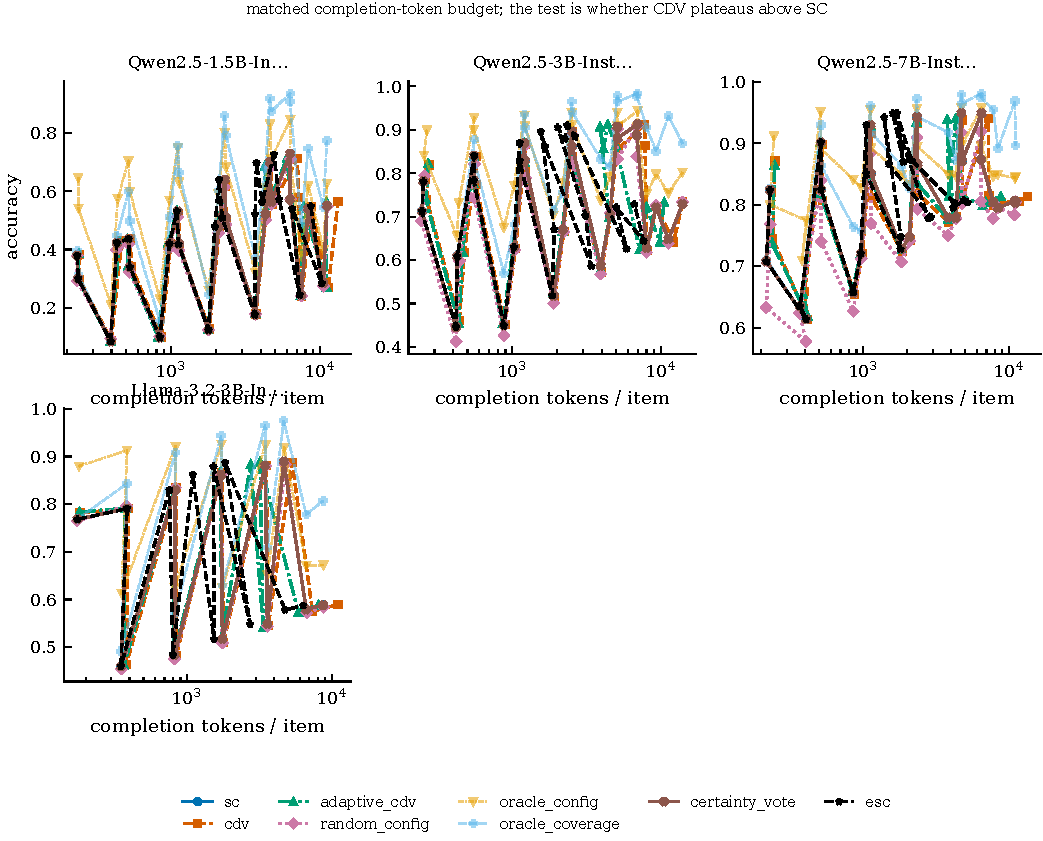
\includegraphics[width=\linewidth]{figures/fig5_cdv_vs_sc.pdf}
\caption{CDV vs.\ self-consistency under token-matched budgets (F5).}
\label{fig:cdv}
\end{figure}

\subsection{Held-out selection and seed-matched controls (C3)}
\label{sec:results-selection}

\paragraph{Setup.}
Pre-specified \texttt{conditional\_diversify} (threshold fit on train; five
overlapping $40\%$ holdouts): use $c_0$ when its vote margin $\ge\tau$, else
plurality over per-config modes.

\paragraph{Apparent gain (14 cells).}
Vs.\ SC@$N$: mean ${\approx}{+}2.3$\,pp (cell-bootstrap CI
$[{+}1.1,{+}3.7]$). Beats val-selected single-config and uniform mode-vote on
average.

\paragraph{Seed-matched controls (6 cells today).}
\label{para:c3-controls}
$c_0$ seeds $\{0,1,2\}$ exist for Qwen$\times$\{GSM8K, MATH-500\} only---not
Llama or GSM-Symbolic (largest C1 spreads). Replace $\{c_0,c_1,c_2\}$ by $c_0$
seeds and compare to SC@$3N$ (pooled $c_0$ seed samples):
\begin{table}[t]
\centering
\caption{C3 contrasts (pp). Seed controls: six multi-seed cells; CIs are
cell-bootstrap.}
\label{tab:c3-controls}
\resizebox{\linewidth}{!}{%
\begin{tabular}{@{}lrrr@{}}
\toprule
Contrast & $n$ & Mean & 95\% CI \\
\midrule
CD$-$SC (all 14) & 14 & $+2.29$ & $[+1.07,+3.70]$ \\
CD$-$SC (seed 6) & 6 & $+1.58$ & $[+0.42,+2.89]$ \\
CD$-$SC (no-seed 8) & 8 & $+2.82$ & $[+0.94,+4.93]$ \\
Seed-sub$-$SC & 6 & $+2.01$ & $[+0.61,+3.52]$ \\
SC@$3N$$-$SC & 6 & $+1.20$ & $[+0.22,+2.18]$ \\
CD$-$seed-sub & 6 & $-0.42$ & $[-1.20,+0.28]$ \\
CD$-$SC@$3N$ & 6 & $+0.39$ & $[-0.11,+0.89]$ \\
\bottomrule
\end{tabular}}
\end{table}
Both key residuals cross zero: we \textbf{cannot distinguish} configs from
seeds at this power. We do \emph{not} claim proven equivalence. A 16-run
seed-expansion queue (Symbolic + Llama, ${\approx}45$ GPU-h) is shipped to
close the eight uncontrolled cells; analysis scripts auto-expand when seeds land.

\paragraph{Independent margin-split.}
Estimating the $c_0$ margin on one half of samples and deciding on the other
half still yields CD$-$SC ${\approx}{+}3.2$\,pp (CI~$[{+}1.4,{+}5.5]$): the
lift is not an artefact of reusing the same draws for margin and vote.

\paragraph{Compute: probe-then-commit tokens.}
Always sample $c_0$; add $c_1$/$c_2$ only when margin${<}\tau$. Mean over 14
cells: early-exit fraction ${\approx}0.74$; token cost ${\approx}1.60\times$
SC@$N$ and ${\approx}0.53\times$ always-3. \cref{fig:token-pareto} places SC,
ESC, certainty-weighted voting, and CDV on an accuracy-vs-actual-tokens curve:
ESC matches SC accuracy at substantially fewer tokens; equal-budget CDV does
not dominate the frontier.

\begin{figure}[t]
\centering
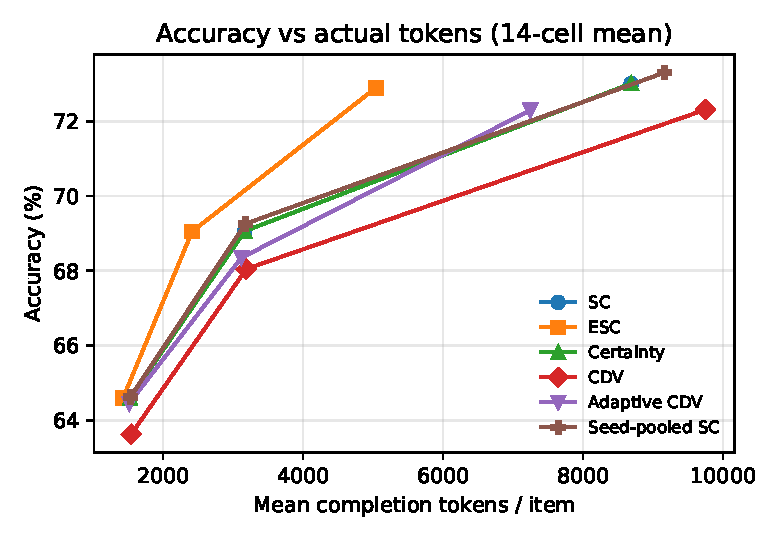
\includegraphics[width=\linewidth]{figures/fig_token_pareto.pdf}
\caption{Accuracy vs.\ mean completion tokens (14-cell mean; offline pool).}
\label{fig:token-pareto}
\end{figure}

\paragraph{Quality-matched ablations.}
Dropping weak $c_2$ raises CD$-$SC to ${\approx}{+}3.3$\,pp; quality-weighted
CD yields only ${\approx}{+}0.7$\,pp. Sample-level mixture of the 3-config pool
does \emph{not} beat SC@$3N$ on seed cells ($\Delta{\approx}{-}0.3$\,pp). Thus
$c_2$ is a quality confound for unweighted pooling, not free diversity.

\paragraph{Seed-null oracles.}
$c_0$ seeds as fake configs: mean oracle gap ${\approx}4.5$\,pp, matching
cross-config plug-in oracles (\cref{tab:seed-null}).

\begin{table}[t]
\centering
\caption{Seed-null plug-in oracle gap (pp): $\max_{\mathrm{seed}}-\mathrm{seed}\,0$.}
\label{tab:seed-null}
\small
\begin{tabular}{llrr}
\toprule
Model & Dataset & Gap & $n$ \\
\midrule
1.5B & GSM8K & 11.1 & 199 \\
3B & GSM8K & 2.5 & 200 \\
7B & GSM8K & 1.0 & 200 \\
1.5B & MATH-500 & 6.5 & 199 \\
3B & MATH-500 & 3.5 & 200 \\
7B & MATH-500 & 2.5 & 200 \\
\midrule
Mean & & 4.5 & \\
\bottomrule
\end{tabular}
\end{table}

\paragraph{Implication.}
Withdraw elicitation-headroom claims. Report seed-null, seed-substitution,
SC@$kN$, margin-split, and actual-token cost---on the \emph{same} cell set as
the headline gain---before attributing multi-prompt lifts to elicitation.

\subsection{Mode reordering (Q2)}
\label{sec:results-reorder}

Pairs are unordered combinations evaluated in lexicographic order
$(c_A{\to}c_B)$ (so rates are \emph{not} symmetric by construction). Mean over
pairs: reorder $21.6\%$, corrective $4.0\%$, destructive $6.4\%$
(\cref{fig:reorder}; \cref{prop:margin-gate}). Reorderings concentrate on small
source margins. This analysis is descriptive---not a proven causal account of
CDV---and partly reflects that stronger configs appear earlier in the lex order.
Depth persistence: transition-persistence CSV on O2 cells.

\begin{figure}[t]
\centering
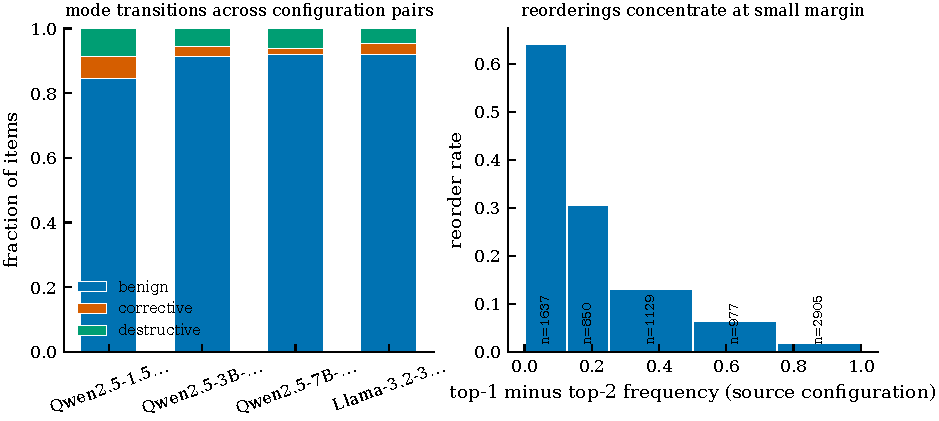
\includegraphics[width=\linewidth]{figures/fig6_reordering.pdf}
\caption{Mode reordering: corrective vs.\ destructive (F6).}
\label{fig:reorder}
\end{figure}

\subsection{Variance, transfer, precision, downstream (Q4)}
\label{sec:results-support}

VB-GLMM decomposition (\cref{fig:variance}; Table~T3): item and model dominate;
item\,$\times$\,config share is $0.82\%$ on GSM8K
(CI $[0.81\%,1.74\%]$) and $0.32\%$ on MATH-500 (CI $[0.22\%,0.65\%]$), so
\textbf{P1 is unsupported}---ceiling gaps need not imply a large crossed variance
share when mass shifts near the decision boundary. Transfer/overlap panels and
Symbolic spreads are in \cref{app:extra-figs} (F2, F3, F7) and Tables~T4--T6.
GSM-Symbolic lacks a fully crossed four-model design (no Llama on that arm), so
its variance block is omitted.

\paragraph{Precision (P7; exploratory until $\rdis$ lands).}
On MATH-500, 4-bit drops mean $\pmode$ sharply vs.\ fp16
($\Delta\approx -16$\,pp pooled in T7) while item\,$\times$\,config share moves by
${<}0.2$\,pp. Without 4-bit $\rdis$, P7 remains \textbf{unsupported}
(\cref{fig:precision}); we do not treat share-only agreement as confirmatory.

\paragraph{Downstream (P6).}
Table~T6: where adaptive gains are reportable, transferring difficulty from
another configuration often retains ${<}1$ of the aware-allocation gain
(sometimes negative on 1.5B GSM8K; $\approx 0.94$ on 3B GSM8K).

% ============================================================================
\section{Discussion}
\label{sec:analysis}
% ============================================================================

\paragraph{Joint outcome.}
Pooling fails to lift SC; a margin-aware rule appears to help vs.\ SC@$N$; on
the six controlled cells that help is not distinguishable from seed-matched
extra samples. That conjunction is the paper---not a positive prompt-selection
method. The eight uncontrolled cells caution against over-generalising the
denoising attribution.

\paragraph{On reordering and CDV.}
Mean corrective / destructive rates are $4.0\%$ / $6.4\%$
(\cref{fig:reorder}), but the pair ordering is lexicographic and asymmetric, so
these rates are descriptive---not a causal account of C2. Oracle rows in
Table~T5 are plug-in maxima inflated by the same finite-$N$ noise the seed null
exposes; we do not read them as untouched elicitation headroom.

\paragraph{Where C1 is strong vs.\ weak.}
Spreads are largest under distribution shift (GSM-Symbolic) and on some GSM8K
rungs; MATH-500 aggregate ranges stay $\le 3$\,pp. We treat Symbolic as a
ceiling stress test and MATH-500 as the place where, for our core prompts,
ceilings are comparatively stable. Scale is non-monotone (3B GSM8K $0.5$\,pp
vs.\ 1.5B/7B $6.5$\,pp).

\paragraph{Small variance shares are compatible with C1.}
GLMM item\,$\times$\,config shares ${<}1\%$ (point) do not contradict
Table~\ref{tab:main-acc}: reordering near the decision boundary can move maj@$N$
without inducing a large crossed random effect of the kind BrittleBench/TEE
emphasise on deterministic suites. Variance decomposition remains supporting
measurement, not the headline.

\paragraph{What we are not claiming.}
We do not claim that prompt selection recovers elicitation headroom, that CDV
is equivalent to SC, or frontier generality. We claim a careful negative on
equal-budget pooling and a measurement result: without seed/depth controls,
multi-prompt ``selection'' gains are easy to misattribute.

\section{Limitations}
\label{sec:limitations}
% ============================================================================

\begin{itemize}\itemsep1pt
  \item \textbf{Scale.} Models fit on $\le 2\times$16\,GB GPUs; frontier /
    reasoning-specialised behaviour may differ.
  \item \textbf{Configuration sample.} Three core prompts are not a census;
    C2 is for equal-budget CDV on $\{c_0,c_1,c_2\}$; C3 policies are exactly the
    held-out selectors we implement (not an exhaustive search over all rules).
  \item \textbf{Semantics preservation} is argued via axes that avoid rewriting
    the problem; residual role / length / format shift is possible. We log
    per-config extraction failures (T1/T2).
  \item \textbf{Finite $N$ / plug-in modes.} $N{=}24$ (mostly); O2 uses $N{=}64$
    on selected MATH-500 3B cells. Depth-stability and transition-persistence
    tables quantify mode-label sensitivity to sampling depth.
  \item \textbf{Uncertainty / power.} Primary contrasts use item-clustered
    bootstrap CIs ($B{=}1000$) and VB-GLMM shares. CDV$-$SC TOST at
    $\delta{=}1$\,pp is inconclusive: we establish no positive lift, not
    equivalence. Some VB fits emit non-convergence warnings; we report shares
    alongside moment estimates in T3.
  \item \textbf{Benchmarks.} MATH-500/Symbolic lead; GSM8K is secondary
    (contamination). Symbolic lacks a fully crossed Llama arm.
  \item \textbf{Canonicalisation.} Symbolic checker errors enter $\pmode$; we
    log extraction failures.
  \item \textbf{P7.} 4-bit $\rdis$ required before calling P7 supported
    (exploratory until then).
  \item \textbf{C3 controls.} Seed-substitution / SC@$3N$ cover six Qwen
    GSM8K/MATH-500 cells (three seeds). Config$-$seed CI
    $[{-}1.20,{+}0.28]$\,pp and config$-$SC@$3N$ CI $[{-}0.11,{+}0.89]$\,pp
    both cross zero. Llama and GSM-Symbolic seeds are queued
    (\texttt{configs/seed\_expansion/}; ${\approx}45$ GPU-h for P0) but not
    yet graded. Probe-then-commit token ratios are offline estimates.
  \item \textbf{Seed null / P4.} Oracle gaps and seed-permutation P4 use three
    $c_0$ seeds; deeper seeds ($\{3,4\}$) are queued as P1.
\end{itemize}

% ============================================================================
\section{Conclusion}
\label{sec:conclusion}
% ============================================================================

Equal-budget prompt pooling does not beat self-consistency under our CIs.
A margin-aware aggregator can beat SC@$N$, but on controlled cells we cannot
distinguish that lift from seed-substitution / SC@$3N$; probe-then-commit
still costs ${\approx}1.6\times$ SC@$N$ tokens. Plug-in oracles and uncalibrated
P4 spreads are inflated by finite-$N$ noise. The practical message is
methodological: do not ensemble prompts by default, and do not credit
multi-prompt selectors without seed-null, seed-substitution, SC@$kN$,
margin-split, and actual-token controls on the \emph{same} cell set as the
headline gain.

\section*{Impact Statement}
This work studies evaluation and test-time aggregation for open-weight math
reasoning models. Potential impacts are improved honesty in reporting reasoning
benchmarks and more careful use of difficulty labels in curricula. We do not
release new high-risk capabilities; experiments are inference-only on public
benchmarks. Misuse risk is low relative to generative systems; the main risk is
over-interpreting C2 as ``prompts never matter'' (contradicted by C1) or
over-interpreting C3 as elicitation recovery (contradicted by seed-substitution
and SC@$3N$).

\section*{Reproducibility Statement}
All experiments are inference-only on open-weight models. Harness, configs, and
analysis code accompany the submission; artefacts reproduce via
\texttt{scripts/split\_precision.py} then
\texttt{python -m src.analysis.paper}. Exact run inventory: \texttt{tab1\_setup.csv}.
Figure/table files: \texttt{paper/figures/}, \texttt{paper/tables/}.

\bibliography{references}
\bibliographystyle{icml2027}

\clearpage
\appendix
\section{Additional Figures}
\label{app:extra-figs}

\begin{figure}[h]
\centering
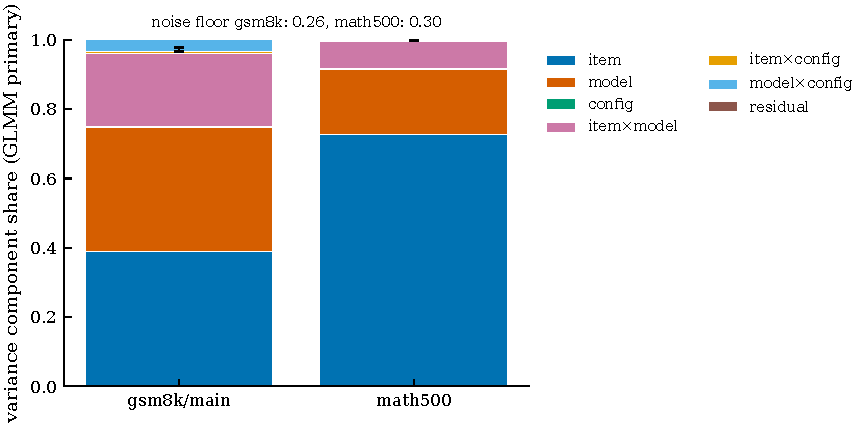
\includegraphics[width=0.85\linewidth]{figures/fig1_variance_components.pdf}
\caption{Variance components (F1; VB-GLMM shares with moment comparison in T3).}
\label{fig:variance}
\end{figure}

\begin{figure}[h]
\centering
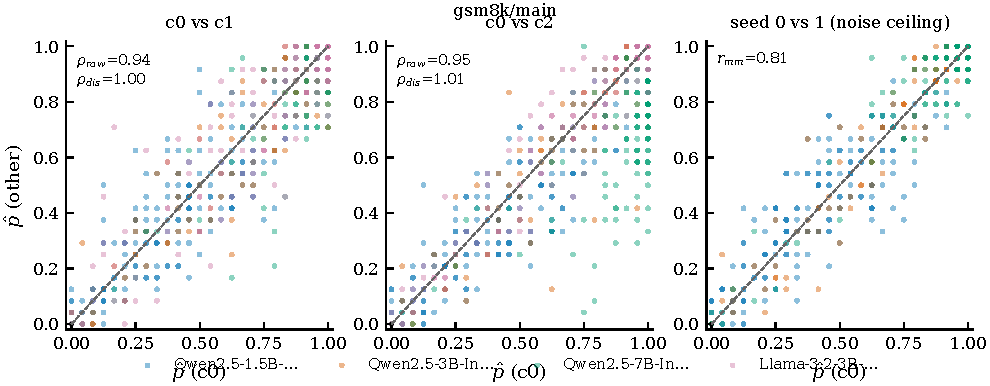
\includegraphics[width=0.85\linewidth]{figures/fig2_transfer_scatter.pdf}
\caption{Difficulty transfer across configurations (F2).}
\label{fig:transfer}
\end{figure}

\begin{figure}[h]
\centering
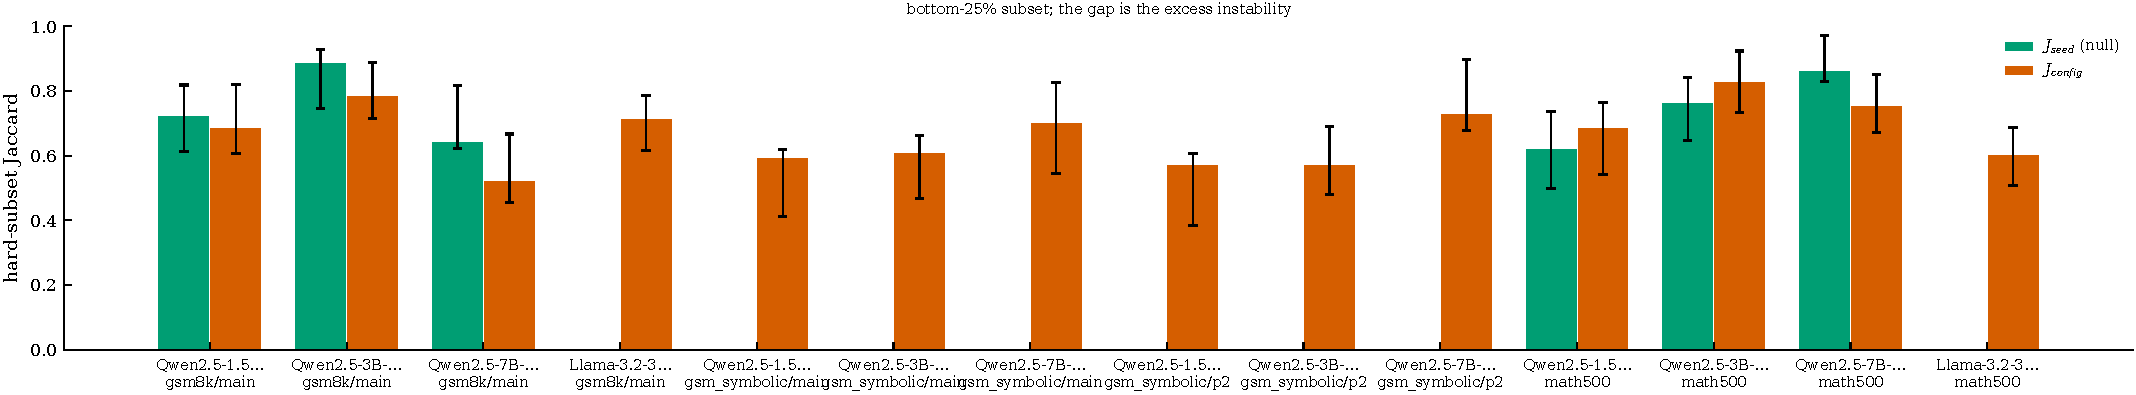
\includegraphics[width=0.85\linewidth]{figures/fig3_hard_subset_overlap.pdf}
\caption{Hard-subset overlap across configs vs.\ seeds (F3).}
\label{fig:overlap}
\end{figure}

\begin{figure}[h]
\centering
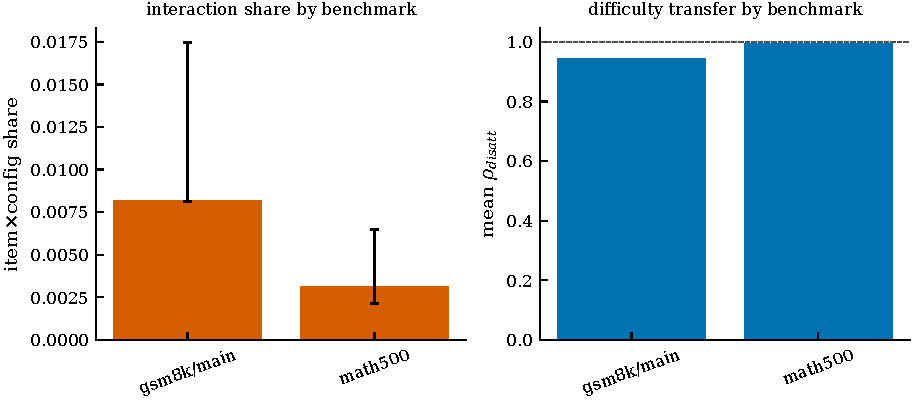
\includegraphics[width=0.85\linewidth]{figures/fig7_shift.pdf}
\caption{GSM-Symbolic shift / ceiling spreads (F7).}
\label{fig:shift}
\end{figure}

\begin{figure}[h]
\centering
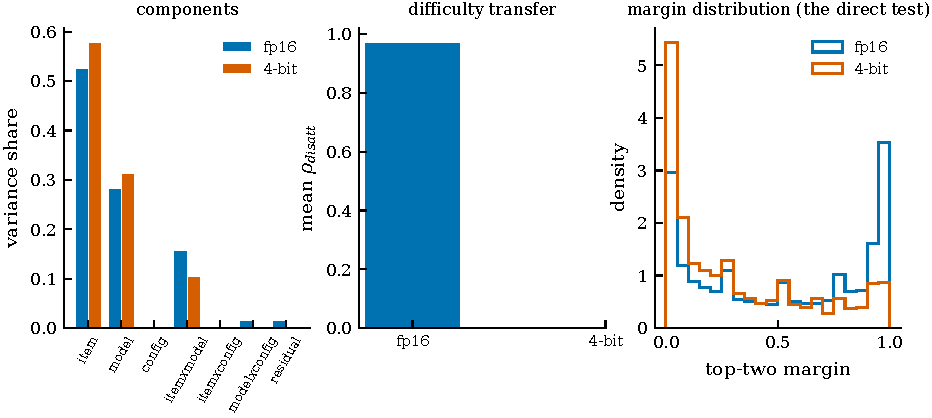
\includegraphics[width=0.85\linewidth]{figures/fig8_precision_control.pdf}
\caption{fp16 vs.\ 4-bit control (F8).}
\label{fig:precision}
\end{figure}

\section{Extended Related Work}
\label{app:related}
\label{sec:related}
% ============================================================================

\subsection{Chain-of-thought and its structural variants}

Chain-of-thought prompting~\citep{wei2022cot} and its zero-shot
form~\citep{kojima2022zeroshot} established that eliciting intermediate steps
improves reasoning accuracy, and self-consistency~\citep{wang2023selfconsistency}
established that sampling several chains and taking a plurality vote improves
it further. A family of structural elaborations followed:
least-to-most decomposition~\citep{zhou2023leasttomost}, tree-~\citep{yao2023tot}
and graph-structured~\citep{besta2024got} search over partial thoughts, and
program-mediated reasoning that offloads arithmetic to an
interpreter~\citep{chen2023pot,gao2023pal}. Later work tempered the picture:
\citet{sprague2025tocot} find that CoT's benefit is concentrated on
mathematical and symbolic tasks and is small or negative elsewhere, and much of
the apparent advantage of elaborate search structures narrows once sampling
budget is matched. \textbf{What remains unresolved:} the community still lacks
a principled account of \emph{which} items benefit from which structure, and
almost all such accounts are stated in terms of a per-item difficulty that can
shift under elicitation and under finite-$N$ mode estimation noise.

\subsection{Test-time compute scaling and its ceilings}

Our benchmarks are \textbf{MATH-500}~\citep{math500} (headline) and
GSM-Symbolic~\citep{mirzadeh2025gsmsymbolic}, with GSM8K~\citep{cobbe2021gsm8k}
as a secondary replicate. Verifier-reranked sampling~\citep{cobbe2021gsm8k}, process
supervision~\citep{lightman2024verify,uesato2022process,wang2024mathshepherd},
and compute-optimal allocation between sequential revision and parallel
sampling~\citep{snell2024scaling,wu2024inference} form the backbone of
test-time scaling; \citet{brown2024monkeys} showed that coverage---the
probability that at least one of $n$ samples is correct---keeps rising over
orders of magnitude of $n$, while plurality voting and learned reward models
plateau. \citet{muennighoff2025s1} showed that a very simple budget-forcing
scheme captures much of the benefit. Surveys now organise the
area along what/how/where/how-well axes~\citep{zhang2025ttssurvey} and by
subproblem topology~\citep{subproblemsurvey2025}, and a large matched-condition
study finds that no single strategy dominates across models and difficulty
regimes~\citep{artofscaling2025}.

The most directly relevant recent development is the explanation of the
plateau. \citet{brown2024monkeys} showed coverage keeps rising while plurality
voting plateaus; subsequent work formalises a \emph{modal ceiling}:
plurality voting converges to the mode, so selection accuracy saturates at
$\pmode$; the gap to rising coverage is the \emph{identifiability gap}
\citep{blendasc2025,certifiedsc2025,samplecomplexity2025}.
\textbf{What remains unresolved:}
all of this conditions on a per-item answer distribution under a \emph{fixed}
elicitation setting. \citet{bay2026modal} estimate run-to-run variance within a
configuration ($\rho_w \approx 0$) but never vary the prompt; whether $\pmode$
is configuration-relative is the step we test.

\subsection{Prompt sensitivity and variance decomposition}
\label{sec:related-prompt}

Three 2026 lines establish that per-item outcomes are prompt-attributable and
that evaluation pipelines must model crossed facets. \textbf{BrittleBench}
\citep{brittlebench2026} decomposes binary correctness variance into task
difficulty and semantics-preserving prompt sensitivity on an item\,$\times$\,perturbation
matrix; inference is deterministic (log-prob scoring), so the inference-variance
term vanishes. \textbf{TEE} \citep{tee2026} fits crossed random effects---including
item\,$\times$\,prompt---by REML and uses decision studies on aggregate benchmark
scores. \textbf{PromptEval} \citep{prompteval2024} estimates performance
distributions across prompt templates with an IRT-style model on the joint
(item, template) matrix. Earlier aggregate work
\citep{sclar2024formatspread,mizrahi2024multiprompt,alzahrani2024leaderboard}
showed format and template choice move rankings by large margins.

\textbf{What remains unresolved} is the intersection with \emph{sampled}
chain-of-thought on free-generation math and with the \emph{mode}. BrittleBench
does not report $\pmode$, reorder rates, or CDV; TEE's estimand is
$\mathrm{Var}(\hat\theta)$ at benchmark scale---item\,$\times$\,prompt is a
nuisance that averages away in aggregate CIs, whereas adaptive test-time compute,
hard-subset curation, and IRT consumers use \emph{per-item} parameters one at a
time. \citet{facetnoise2026,cyclicjudge2026} show that under G-theory facet decompositions,
repeats are the cheap facet and paraphrases/models buy more reliability per
query---the allocation-theoretic sibling of ``i.i.d.\ resampling cannot move the
plateau,'' but on brand sentiment without modes or reasoning. \citet{hardunreached2026}
establish unstable hardness labels along the stochastic-vs-deterministic axis;
we study the \emph{configuration} axis and whether it reaches the selection
bottleneck. Adjacent aggregation devices---paraphrase
voting~\citep{paraconsistency2024,zhou2024paraphrase}---are baselines, not the
measurement target.

\subsection{Long chain-of-thought, RL for reasoning, and the elicitation debate}

Reasoning-specialised models trained with reinforcement learning on verifiable
rewards~\citep{deepseekr1_2025,shao2024deepseekmath} produce long
chains-of-thought and large gains, and distillation transfers much of the
behaviour into small models with remarkably little
data~\citep{muennighoff2025s1,ye2025limo}. A pointed debate followed about what
RL actually contributes. \citet{yue2025rlvr} argue via pass@$k$ analysis that
RLVR largely sharpens the base model's existing distribution rather than
extending its reach, and \citet{diversitycollapse2025} formalise a related
bias--variance decomposition of pass@$k$, showing that supervised finetuning
improves pass@1 while collapsing generation diversity and degrading pass@$k$,
and that weight interpolation partially recovers both. Theoretically,
self-improvement has been framed as \emph{sharpening} a fixed base
policy~\citep{huang2025sharpening}, and inference-time methods have been
recast as sharpening the answer marginal
directly~\citep{marginalsharpening2026}. \textbf{What remains unresolved:} the
sharpening framing implies that the ordering of candidate answers is doing all
the work, but the stability of that ordering---under scale, under
post-training, and under elicitation---has not been measured. Our
mode-reordering analysis (\cref{sec:results-reorder}) is the missing
measurement for the elicitation axis.

\subsection{Faithfulness, premature commitment, and what the chain is for}

A parallel literature asks whether the chain reflects the computation.
\citet{turpin2023unfaithful} show that models silently follow biasing features
in the context while producing unrelated rationales;
\citet{lanham2023measuring} introduce the truncation and corruption probes that
have become standard; and \citet{lyu2023faithful} propose constrained
formulations that are faithful by construction. Latent-space variants ask
whether the tokens are needed at
all~\citep{hao2024coconut,pfau2024filler,goyal2024pause}. Recent work sharpens
the commitment question: \citet{prematureconfidence2026} probe at evenly spaced
truncation points, define a premature-confidence score from the resulting
confidence trajectory, show it predicts logical flaws, and mitigate it with a
shaped RL objective; \citet{precotprobe2026} show that a linear probe on
pre-CoT activations predicts the final answer with high AUC and that the
direction is causal under steering. \citet{matcha2025} show the converse
decoupling---answers that stay correct while the rationale collapses under
imperceptible input perturbation. \textbf{What remains unresolved:} these
results establish that a model often has an answer in mind early, but they do
not connect that to the \emph{selection} bottleneck at the heart of test-time
scaling. Early commitment is one candidate mechanism for genuine mode shifts;
our seed-null and seed-substitution results show that many apparent shifts are
also consistent with finite-$N$ estimation noise, so the mechanism remains open.

\subsection{Efficiency, overthinking, and adaptive compute}

Reasoning models overspend on easy items~\citep{overthinking2024} and
under-explore on hard ones~\citep{underthinking2025}; surveys catalogue the
resulting efficiency
literature~\citep{stopoverthinking2025}. Length-controlled policy
optimisation~\citep{l1_2025} and budget-forcing~\citep{muennighoff2025s1} give
explicit control over chain length. On the parallel axis,
adaptive-consistency~\citep{aggarwal2023adaptive} and early-stopping
self-consistency~\citep{li2024esc} halt when the vote is decided;
Certaindex/Dynasor~\citep{fu2024certaindex} generalise this to an
algorithm-agnostic ``answer stabilisation'' signal used for scheduling;
Blend-ASC~\citep{blendasc2025} allocates samples across questions to optimise
sample efficiency; \citet{certifiedsc2025} provide sequential certificates; and
\citet{adaptivettc2026} study difficulty-conditioned budget allocation directly.
\textbf{What remains unresolved:} every one of these estimates a per-item
quantity in one setting and consumes it in another, and none validates that the
estimate transfers. This is the applied consequence we measure.

\subsection{Robustness, perturbation, and the reasoning-versus-memorisation debate}

\citet{mirzadeh2025gsmsymbolic} introduced templated variants of GSM8K and
reported both high variance across instantiations of the same template and a
large drop when an irrelevant clause is added (GSM-NoOp), arguing for
pattern-matching over formal reasoning. Contamination
audits~\citep{zhang2024gsm1k}, counterfactual
evaluation~\citep{wu2024reciting}, premise-order
effects~\citep{chen2024premise} and the reversal
curse~\citep{berglund2024reversal} point the same direction, while
compositionality analyses~\citep{dziri2023faithfate} give a mechanistic account
of multi-step failure. The debate is live: puzzle-complexity critiques and
their rebuttals continue, and 2026 replications of GSM-NoOp on frontier models
suggest that a substantial part of the original effect reflects models
reasonably treating ambiguous clauses as informative rather than failing to
reason. Follow-up
work finds that program-mediated reasoning does not repair GSM-Symbolic
robustness~\citep{reasoningcodeboth2026}. \textbf{What remains unresolved:}
these studies compare accuracy across perturbations of the \emph{problem}. Ours
holds the problem fixed and perturbs only the \emph{elicitation}, isolating a
source of instability that cannot be blamed on the item---subject to the
seed-matched controls in the main text.

\subsection{Self-correction, verification, and aggregation beyond frequency}

Iterative refinement with self-generated feedback~\citep{madaan2023selfrefine}
and multi-agent debate~\citep{du2024debate} were early attempts to convert extra
inference into extra accuracy without a verifier, but intrinsic self-correction
without external feedback does not reliably improve
reasoning~\citep{huang2024cannotselfcorrect,kamoi2024whencan}, which is part of
why the field turned to verifiers and to better aggregation. Beyond plain
plurality voting there is now a dense cluster: universal
self-consistency~\citep{chen2023universal}, program-verified
voting~\citep{prove2024}, semantic weighting of reasoning
paths~\citep{weightedreasoning2024}, confidence-informed voting and its
efficient variant~\citep{veccisc2026}, learned rerankers over answer-level
features~\citep{risc2026}, radial consensus scoring for
best-of-$N$~\citep{rcs2026}, and best-of-majority
hybrids~\citep{bestofmajority2025}.
Diversity-side interventions are covered in
\cref{sec:related-prompt}. \textbf{What remains unresolved:}
this literature searches for a better \emph{selector} given a fixed sample
pool. We ask a prior question---what determines the pool's mode in the first
place---and show that the answer includes a factor the selector literature
treats as fixed. The strongest of these methods are our baselines.

\subsection{Uncertainty, calibration, and evaluation methodology}

Confidence signals for reasoning include self-evaluated
correctness~\citep{kadavath2022know}, semantic
entropy~\citep{kuhn2023semantic,farquhar2024semantic}, verbalised
confidence~\citep{lin2022teaching,tian2023just}, and vote share itself. On the
evaluation side, the field has become considerably more careful:
\citet{miller2024errorbars} argues for routine interval reporting,
\citet{hochlehnert2025sober} document how much of recent reported progress on
small reasoning benchmarks is seed variance, \citet{dontpassk2025} propose
Bayesian posterior reporting in place of pass@$k$,
\citet{coverattau2025} show that pass@$k$ is biased toward low-reliability
``lucky hits'' and propose a reliability-controlled alternative, and
\citet{falsepositives2025} show that final-answer matching admits false
positives at a rate that materially lowers the true inference-scaling ceiling.
Psychometric approaches fit item difficulty explicitly and use it for adaptive
testing and routing~\citep{atlas2025,irtnet2025,irtrouter2025,psnirt2026}, and
\citet{kim2025correlated} show that errors are strongly correlated across
models, capping ensembles---an effect formalised as a co-failure
ceiling~\citep{cofailure2026}. \textbf{What remains unresolved:} the
psychometric line assumes a unidimensional item difficulty and validates it
largely on non-reasoning benchmarks. We test that assumption where it is most
consequential, and we adopt the evaluation hygiene this literature demands
throughout.

% ============================================================================


\end{document}
